\documentclass[a4paper,14pt,oneside,final]{extarticle}
\usepackage[top=2cm, bottom=2cm, left=3cm, right=1cm]{geometry}
\usepackage{scrextend}

\usepackage[T2A,T1]{fontenc}
\usepackage[ukrainian,russian,english]{babel}
\usepackage{tempora}
\usepackage{fontspec}
\setmainfont{tempora}

% Зачем: Отключает использование изменяемых межсловных пробелов.
% Почему: Так не принято делать в текстах на русском языке.
\frenchspacing

\usepackage{indentfirst}
\setlength{\parindent}{1.25cm}
\renewcommand{\baselinestretch}{1.5}

% Header
\usepackage{fancyhdr}
\pagestyle{fancy}
\fancyhead{}
\fancyfoot{}
\fancyhead[R]{\small \selectfont \thepage}
\renewcommand{\headrulewidth}{0pt}

% Captions
\usepackage{chngcntr}
\counterwithin{figure}{section}
\counterwithin{table}{section}
\usepackage[tableposition=top]{caption}
\usepackage{subcaption}
\DeclareCaptionLabelFormat{gostfigure}{Рисунок #2}
\DeclareCaptionLabelFormat{gosttable}{Таблиця #2}
\DeclareCaptionLabelSeparator{gost}{~---~}
\captionsetup{labelsep=gost}
\captionsetup[figure]{labelformat=gostfigure}
\captionsetup[table]{labelformat=gosttable}
\renewcommand{\thesubfigure}{\asbuk{subfigure}}

% Sections
\usepackage[explicit]{titlesec}
\newcommand{\sectionbreak}{\clearpage}

\titleformat{\section}
  {\centering}{\thesection \quad}{0pt}{\MakeUppercase{#1}}
\titleformat{\subsection}[block]
  {\bfseries}{\thesubsection \quad #1}{0cm}{}

\titlespacing{\section} {0cm}{0cm}{21pt}
\titlespacing{\subsection} {\parindent}{21pt}{0cm}
\titlespacing{\subsubsection} {\parindent}{0cm}{0cm}

% Lists
\usepackage{enumitem}
\renewcommand\labelitemi{--}
\setlist[itemize]{noitemsep, topsep=0pt, wide}
\setlist[enumerate]{noitemsep, topsep=0pt, wide, label=\arabic*}
\setlist[description]{labelsep=0pt, noitemsep, topsep=0pt, leftmargin=2\parindent, labelindent=\parindent, labelwidth=\parindent, font=\normalfont}

% Toc
\usepackage{tocloft}
\tocloftpagestyle{fancy}
\renewcommand{\cfttoctitlefont}{}
\setlength{\cftbeforesecskip}{0pt}
\renewcommand{\cftsecfont}{}
\renewcommand{\cftsecpagefont}{}
\renewcommand{\cftsecleader}{\cftdotfill{\cftdotsep}}

\usepackage{float}
\usepackage{pgfplots}
\usepackage{graphicx}
\usepackage{multirow}
\usepackage{amssymb,amsfonts,amsmath,amsthm}
\usepackage{csquotes}

\usepackage{listings}
\lstset{basicstyle=\footnotesize\ttfamily,breaklines=true}
\lstset{language=Matlab}

\usepackage[
	backend=biber,
	sorting=none,
	language=auto,
	autolang=other
]{biblatex}
\DeclareFieldFormat{labelnumberwidth}{#1}


\newcommand{\labnumber}{1} % first lab
\documentclass[a4paper,14pt,oneside,final]{extarticle}
\usepackage[top=2cm, bottom=2cm, left=3cm, right=1cm]{geometry}
\usepackage{scrextend}

\usepackage[T2A,T1]{fontenc}
\usepackage[ukrainian,russian,english]{babel}
\usepackage{tempora}
\usepackage{fontspec}
\setmainfont{tempora}

% Зачем: Отключает использование изменяемых межсловных пробелов.
% Почему: Так не принято делать в текстах на русском языке.
\frenchspacing

\usepackage{indentfirst}
\setlength{\parindent}{1.25cm}
\renewcommand{\baselinestretch}{1.5}

% Header
\usepackage{fancyhdr}
\pagestyle{fancy}
\fancyhead{}
\fancyfoot{}
\fancyhead[R]{\small \selectfont \thepage}
\renewcommand{\headrulewidth}{0pt}

% Captions
\usepackage{chngcntr}
\counterwithin{figure}{section}
\counterwithin{table}{section}
\usepackage[tableposition=top]{caption}
\usepackage{subcaption}
\DeclareCaptionLabelFormat{gostfigure}{Рисунок #2}
\DeclareCaptionLabelFormat{gosttable}{Таблиця #2}
\DeclareCaptionLabelSeparator{gost}{~---~}
\captionsetup{labelsep=gost}
\captionsetup[figure]{labelformat=gostfigure}
\captionsetup[table]{labelformat=gosttable}
\renewcommand{\thesubfigure}{\asbuk{subfigure}}

% Sections
\usepackage[explicit]{titlesec}
\newcommand{\sectionbreak}{\clearpage}

\titleformat{\section}
  {\centering}{\thesection \quad}{0pt}{\MakeUppercase{#1}}
\titleformat{\subsection}[block]
  {\bfseries}{\thesubsection \quad #1}{0cm}{}

\titlespacing{\section} {0cm}{0cm}{21pt}
\titlespacing{\subsection} {\parindent}{21pt}{0cm}
\titlespacing{\subsubsection} {\parindent}{0cm}{0cm}

% Lists
\usepackage{enumitem}
\renewcommand\labelitemi{--}
\setlist[itemize]{noitemsep, topsep=0pt, wide}
\setlist[enumerate]{noitemsep, topsep=0pt, wide, label=\arabic*}
\setlist[description]{labelsep=0pt, noitemsep, topsep=0pt, leftmargin=2\parindent, labelindent=\parindent, labelwidth=\parindent, font=\normalfont}

% Toc
\usepackage{tocloft}
\tocloftpagestyle{fancy}
\renewcommand{\cfttoctitlefont}{}
\setlength{\cftbeforesecskip}{0pt}
\renewcommand{\cftsecfont}{}
\renewcommand{\cftsecpagefont}{}
\renewcommand{\cftsecleader}{\cftdotfill{\cftdotsep}}

\newcommand{\khpistudentgroup}{КН-34г}
\newcommand{\khpistudentname}{Чепурний~А.~С.}

\newcommand{\khpidepartment}{Програмна інженерія та інформаційні технології управління}
\newcommand{\khpititlewhat}{
	Лабораторна робота №\labnumber \\
	з предмету <<Моделювання систем>>
}
\newcommand{\khpititlewho}{
	Виконав: \\
	\hspace*{\parindent} ст. групи \khpistudentgroup \\
	\hspace*{\parindent} \khpistudentname \\
	Перевірила: \\
	\hspace*{\parindent} ст. в. каф. ПІІТУ \\
	\hspace*{\parindent} Єршова~С.~І. \\
	\hspace*{\parindent} ас. каф. ПІІТУ \\
	\hspace*{\parindent} Литвинова~Ю.~С. \\
}



\graphicspath{{figures/}}

\begin{document}
\Ukrainian

\begin{titlepage}

\begin{center}
	МІНІСТЕРСТВО ОСВІТИ І НАУКИ УКРАЇНИ \\
	НАЦІОНАЛЬНИЙ ТЕХНІЧНИЙ УНІВЕРСИТЕТ \\
	«ХАРКІВСЬКИЙ ПОЛІТЕХНІЧНИЙ ІНСТИТУТ» \\[0.5cm]
	Кафедра <<\khpidepartment>> \\
\end{center}

\vspace{6cm}

\begin{center}
	\khpititlewhat
\end{center}

\vspace{3cm}

\begin{addmargin}[10cm]{0cm}
	\khpititlewho
\end{addmargin}

\vspace{\fill}

\begin{center}
	Харків \the\year
\end{center}

\end{titlepage}

\addtocounter{page}{1}

\section*{Organization Domain Modeling}
\subsubsection*{Цель работы}
Знакомство с методом доменного моделирования ODM (Organization Domain Modeling) и инструментарием Eclipse Modeling Framework.

\subsection*{Ход работв}
\begin{enumerate}
    \item Планирование домена (Plan Domain Engineering).
    \item Моделирование домена (Model Domain).
    \item Разработка функционала (Engineer Asset Base).
\end{enumerate}

\subsection{Планирование домена}
\subsubsection{Цели, требования, существующие решения}
Создание системы которая способна моделировать поведение логистических систем дистрибуции.
Система должна быть показывать уровень сервиса логистической системы.

Существующие решения:
AnyLogic, Simcad Logistics.

\subsubsection{Заинтересованные лица}
Пример заинтересованных лиц:
\begin{itemize}
    \item Senior Management;
    \item Project Leaders;
    \item Application Engineers;
    \item Financial Analysts/Accountants.
\end{itemize}
\subsubsection{Доменная область}
Цели проекта:
\begin{itemize}
    \item закончить в срок обозначенный менеджментом;
    \item производить качественный результат на всех этапах -- от планирования и до разработки;
    \item разработать качественную документацию;
    \item успешно внедрить продукт, не превышая запланированный бюджет.
\end{itemize}

Доменная область представляет собой задачу дистрибьюции логистической системы. 
Начальная структура логистической цели вводится пользователем. 
Система должна показать график уровня сервиса смоделированной логистической системы.

Этот домен не включает в себя качественное моделирование спроса людей и изменения их предпочтений.

\subsection{Моделирование домена}
\subsubsection{Сбор информации}

Глосарій проекту:
\begin{enumerate}
    \item Агент \textit{(agent)} --- это сущность, которая наблюдает за окружающей средой и действует в ней, ее поведение рациональное.
    \item Склад \textit{(warehouse)} --- это сложное техническая сооружение, которое состоит из взаимосвязанных элементов, имеет определенную структуру и выполняет ряд функций по преобразованию материальных потоков, а также накопления, переработки и распределения грузов между потребителями.
	\item Запасы гарантийные \textit{(insurance stocks)} предназначены для непрерывного снабжения потребителей в случае непредвиденных обстоятельств: отклонения в периодичности и величине партий поставок от запланированных, изменения интенсивности потребления, задержки поставок и др., является постоянной величиной, зависит от условий выполнения конкретных поставок.
	\item Логистика распределительная \textit{(distribution logistics)} --- отрасль логистики, которая обеспечивает наиболее эффективную организацию распределения продукции, включая систему товародвижения и логистические операции транспортировки, складирования, упаковки и др.
	\item Уровень сервиса \textit{(service level)} --- количественная характеристика соответствия фактических значений показателей качества и количества логистических услуг оптимальным или теоретически возможным значением.
    \item Магазин \textit{(shop)} --- сооружение для розничной продажи товаров.
    \item Биржа \textit{(exchange)} --- сервис, которые предоставляет возможность заключения сделок с товарами.
    \item Запрос \textit{(request)} --- предложение покупки некоторого количества товаров.
    \item Предложение \textit{(proposal)} --- выражение желания продажи некоторого количества товаров.
\end{enumerate}

\subsubsection{Моделирование домена}
Для моделирования домена был использован EMF фреймворк. 
Результат моделирования представлен на рисунке~\ref{fig:model}. 

\begin{figure}[H]
    \centering
    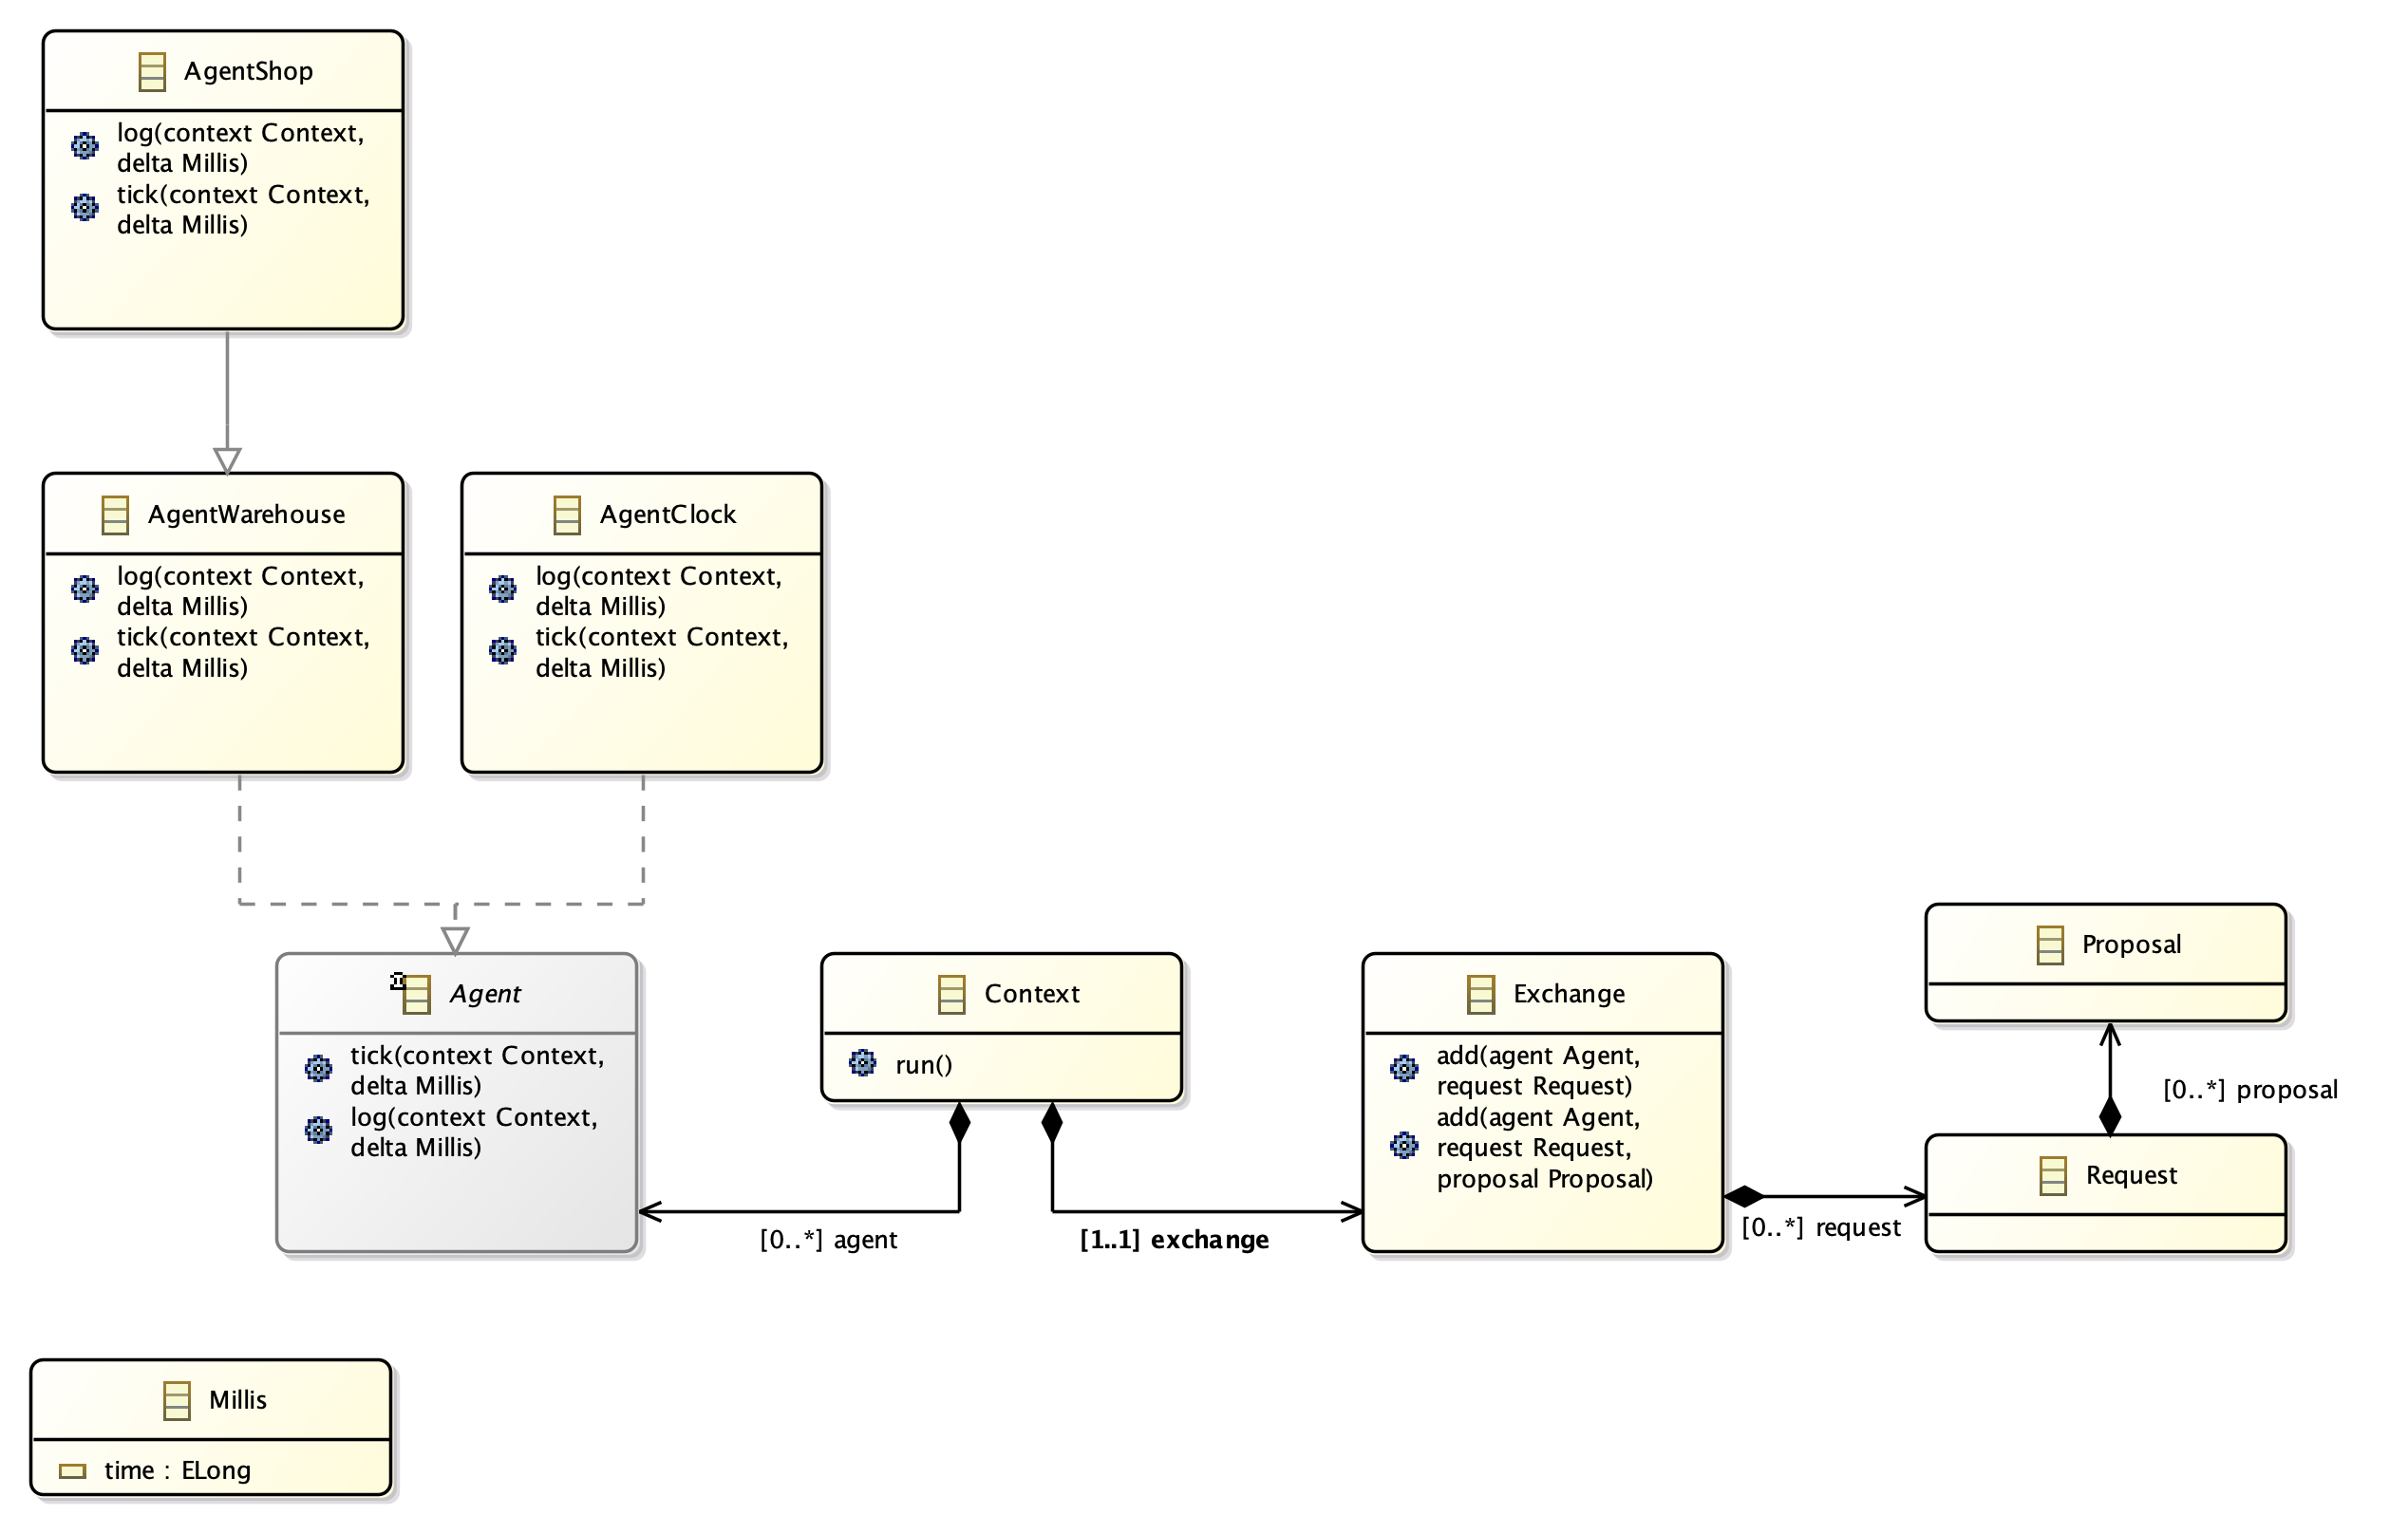
\includegraphics[width=\textwidth]{lab1_2}
    \caption{EMF модель}
    \label{fig:model}
\end{figure}

\subsection{Разработка функционала}
С помощью EMF и модели представленной выше (рисунок~\ref{fig:model}) был сгенерирован исходный код. 
Фрагмент исходного кода представлен ниже:
\begin{lstlisting}
public interface Context extends EObject {

	EList<Agent> getAgent();

	Exchange getExchange();

	void run();

} 

public interface Millis extends EObject {

	long getTime();

	void setTime(long value);

}
\end{lstlisting}

\subsection*{Выводы}
В ходе данной лабораторной работы было проведено знакомство с доменным моделированием ODM. ODM лучше всего подходит для зрелых проектов, которые были разработаны с помощью методов доменной инженерии и являются стабильными.

Было разработана модель представления доменной области <<моделирование логистических систем дистрибуции>> с помощью EMF. 

\end{document}
